% ============================================================
% 第24章 圆 — 人教版九年级上册
% 编译命令：xelatex -interaction=nonstopmode 第24章_圆.tex
% ============================================================
\documentclass[12pt, a4paper]{ctexart}
\usepackage[margin=2.2cm]{geometry}
\usepackage{amsmath, amssymb}
\usepackage{enumitem}
\usepackage{tcolorbox}
\usepackage{booktabs}
\usepackage{array}
\usepackage{fancyhdr}
\usepackage{xcolor}
\usepackage{tikz}
\usepackage{hyperref}
\usepackage{graphicx}
\usepackage{multirow}
\usepackage{pgfplots}
\pgfplotsset{compat=1.18}

% 颜色定义
\definecolor{mainblue}{RGB}{41, 98, 168}
\definecolor{lightblue}{RGB}{230, 240, 255}
\definecolor{tipgreen}{RGB}{34, 139, 87}
\definecolor{lightgreen}{RGB}{235, 250, 240}
\definecolor{warnred}{RGB}{200, 50, 50}
\definecolor{lightred}{RGB}{255, 240, 240}
\definecolor{examorange}{RGB}{210, 120, 20}
\definecolor{lightorange}{RGB}{255, 248, 235}
\definecolor{apppurple}{RGB}{120, 60, 170}
\definecolor{lightpurple}{RGB}{245, 238, 255}

% 页眉页脚
\pagestyle{fancy}
\fancyhf{}
\fancyhead[L]{\small\textcolor{mainblue}{\textbf{人教版九年级上册 \(\cdot\) 第24章 圆}}}
\fancyhead[R]{\small\textcolor{mainblue}{家教讲义}}
\fancyfoot[C]{\small —\ \thepage\ —}
\renewcommand{\headrulewidth}{0.6pt}
\renewcommand{\headrule}{\hbox to\headwidth{\color{mainblue}\leaders\hrule height \headrulewidth\hfill}}
\renewcommand{\footrulewidth}{0pt}

% tcolorbox 样式
\newtcolorbox{knowledgebox}[1][]{%
  colback=lightblue, colframe=mainblue,
  fonttitle=\bfseries\large, title=#1,
  arc=3mm, boxrule=0.8pt,
  left=8pt, right=8pt, top=6pt, bottom=6pt
}

\newtcolorbox{tipbox}[1][]{%
  colback=lightgreen, colframe=tipgreen,
  fonttitle=\bfseries, title=#1,
  arc=2mm, boxrule=0.6pt,
  left=6pt, right=6pt, top=4pt, bottom=4pt
}

\newtcolorbox{warnbox}[1][]{%
  colback=lightred, colframe=warnred,
  fonttitle=\bfseries, title=#1,
  arc=2mm, boxrule=0.6pt,
  left=6pt, right=6pt, top=4pt, bottom=4pt
}

\newtcolorbox{examplebox}[1][]{%
  colback=lightorange, colframe=examorange,
  fonttitle=\bfseries, title=#1,
  arc=3mm, boxrule=0.8pt,
  left=8pt, right=8pt, top=6pt, bottom=6pt
}

\newtcolorbox{appbox}[1][]{%
  colback=lightpurple, colframe=apppurple,
  fonttitle=\bfseries, title=#1,
  arc=3mm, boxrule=0.8pt,
  left=8pt, right=8pt, top=6pt, bottom=6pt
}

\setCJKmainfont{Hiragino Sans GB}
\setCJKsansfont{Heiti SC}

\begin{document}

% ============ 标题页 ============
\begin{center}
{\Huge\bfseries\textcolor{mainblue}{第24章\quad 圆}}\\[12pt]
{\Large\textcolor{gray}{家\ 教\ 讲\ 义}}\\[8pt]
\rule{0.6\textwidth}{1pt}\\[8pt]
{\normalsize 适用：人教版\quad 九年级上册\quad |\quad 课时：10课时}
\end{center}
\vspace{10pt}

% ==============================================================
% 第一部分：知识点讲解
% ==============================================================
\section*{\textcolor{mainblue}{一、知识点讲解}}

% ==================== 24.1 圆的基本概念 ====================
\subsection*{24.1\quad 圆的基本概念}

\begin{knowledgebox}[圆的定义]
在一个平面内，线段 $OA$ 绕它固定的一个端点 $O$ 旋转一周，另一个端点 $A$ 所经过的封闭曲线叫做\textbf{圆}。

固定的端点 $O$ 叫做\textbf{圆心}，线段 $OA$ 叫做\textbf{半径}。

以点 $O$ 为圆心的圆记作 $\odot O$，读作"圆 $O$"。
\end{knowledgebox}

\begin{knowledgebox}[弦与直径]
\begin{itemize}[nosep]
  \item \textbf{弦}：连接圆上任意两点的线段叫做弦。
  \item \textbf{直径}：经过圆心的弦叫做直径。直径是圆中最长的弦，直径 $= 2 \times$ 半径。
\end{itemize}
\end{knowledgebox}

\begin{knowledgebox}[弧]
\begin{itemize}[nosep]
  \item \textbf{弧}：圆上任意两点间的部分叫做弧，记为 $\widehat{AB}$。
  \item \textbf{半圆}：圆的任意一条直径的两个端点把圆分成两条弧，每一条弧都叫做半圆。
  \item \textbf{优弧}：大于半圆的弧（用三个字母表示，如 $\widehat{ACB}$）。
  \item \textbf{劣弧}：小于半圆的弧（用两个字母表示，如 $\widehat{AB}$）。
\end{itemize}
\end{knowledgebox}

\begin{center}
\begin{tikzpicture}[scale=1.0]
  \draw[thick, mainblue] (0,0) circle (2.5);
  \fill (0,0) circle (2pt) node[below left]{$O$};
  % 弦 AB
  \coordinate (A) at ({-2.5*cos(30)}, {-2.5*sin(30)});
  \coordinate (B) at ({2.5*cos(30)}, {-2.5*sin(30)});
  \draw[thick, red] (A) -- (B);
  \fill (A) circle (2pt) node[left]{$A$};
  \fill (B) circle (2pt) node[right]{$B$};
  % 标注弦
  \node[below, red] at (0, -2.1) {弦 $AB$};
  % 直径
  \coordinate (C) at (0, 2.5);
  \coordinate (D) at (0, -2.5);
  \draw[thick, blue] (C) -- (D);
  \fill (C) circle (2pt) node[above]{$C$};
  \fill (D) circle (2pt) node[below]{$D$};
  \node[right, blue] at (0.3, 0) {直径 $CD$};
  % 半径
  \draw[dashed, gray] (0,0) -- (C);
  \node[left, gray] at (0, 1.25) {$r$};
\end{tikzpicture}
\end{center}

\begin{knowledgebox}[圆心角]
\textbf{圆心角}：顶点在圆心的角叫做圆心角。

如图，$\angle AOB$ 就是一个圆心角，它所对的弧是 $\widehat{AB}$，所对的弦是 $AB$。
\end{knowledgebox}

\begin{center}
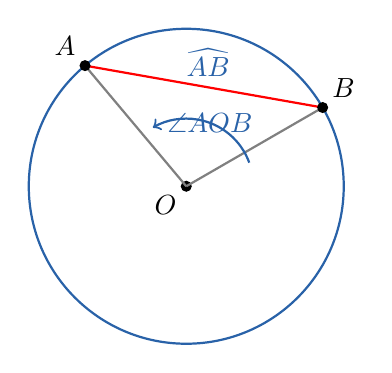
\begin{tikzpicture}[scale=1.0]
  \draw[thick, mainblue] (0,0) circle (2);
  \fill (0,0) circle (2pt) node[below left]{$O$};
  \coordinate (A) at ({2*cos(130)}, {2*sin(130)});
  \coordinate (B) at ({2*cos(30)}, {2*sin(30)});
  \draw[thick, red] (A) -- (B);
  \draw[thick, gray] (0,0) -- (A);
  \draw[thick, gray] (0,0) -- (B);
  \fill (A) circle (2pt) node[above left]{$A$};
  \fill (B) circle (2pt) node[above right]{$B$};
  % 圆心角弧线
  \draw[->, thick, mainblue] (0.8, 0.3) arc (20:120:0.85);
  \node[mainblue] at (0.3, 0.8) {$\angle AOB$};
  % 弧标注
  \node[mainblue] at ({1.6*cos(80)}, {1.6*sin(80)}) {$\widehat{AB}$};
\end{tikzpicture}
\end{center}

\begin{knowledgebox}[圆周角]
\textbf{圆周角}：顶点在圆上，并且两边都与圆相交的角叫做圆周角。

圆周角的特征：
\begin{enumerate}[nosep]
  \item 顶点在圆上；
  \item 两边都与圆相交（即两边都是圆的弦）。
\end{enumerate}
\end{knowledgebox}

\begin{warnbox}[易错提醒：圆心角 vs 圆周角]
\begin{itemize}[nosep]
  \item 圆心角的顶点在\textbf{圆心}，圆周角的顶点在\textbf{圆上}。
  \item 同一条弧可以对应一个圆心角和无数个圆周角。
  \item 不是所有顶点在圆上的角都是圆周角——角的两边必须都与圆相交。
\end{itemize}
\end{warnbox}

% ==================== 24.2 垂径定理 ====================
\subsection*{24.2\quad 垂径定理及其推论}

\begin{knowledgebox}[垂径定理]
\textbf{定理}：垂直于弦的直径平分这条弦，并且平分弦所对的两条弧。

即：在 $\odot O$ 中，直径 $CD \perp$ 弦 $AB$ 于 $E$，则：
\[
AE = BE, \quad \widehat{AC} = \widehat{BC}, \quad \widehat{AD} = \widehat{BD}
\]
\end{knowledgebox}

\begin{center}
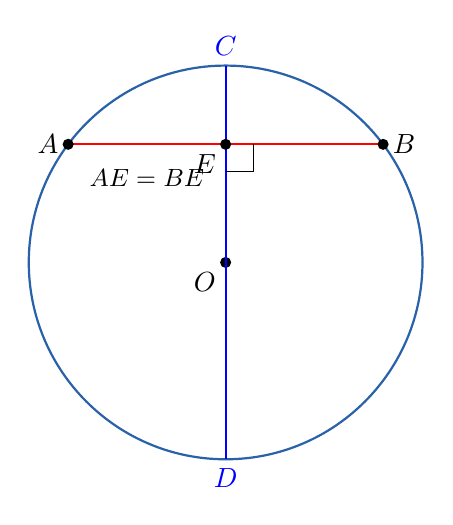
\begin{tikzpicture}[scale=1.0]
  \draw[thick, mainblue] (0,0) circle (2.5);
  \fill (0,0) circle (2pt) node[below left]{$O$};
  % 直径 CD
  \coordinate (C) at (0, 2.5);
  \coordinate (D) at (0, -2.5);
  \draw[thick, blue] (C) -- (D);
  \node[above, blue] at (C) {$C$};
  \node[below, blue] at (D) {$D$};
  % 弦 AB (水平)
  \coordinate (A) at (-2, 1.5);
  \coordinate (B) at (2, 1.5);
  \coordinate (E) at (0, 1.5);
  \draw[thick, red] (A) -- (B);
  \fill (A) circle (2pt) node[left]{$A$};
  \fill (B) circle (2pt) node[right]{$B$};
  \fill (E) circle (2pt) node[below left]{$E$};
  % 垂直标记
  \draw (0, 1.15) -- (0.35, 1.15) -- (0.35, 1.5);
  % 标注
  \node[below, font=\small] at (-1, 1.3) {$AE = BE$};
\end{tikzpicture}
\end{center}

\begin{knowledgebox}[垂径定理的推论]
\textbf{推论}：平分弦（不是直径）的直径垂直于弦，并且平分弦所对的两条弧。

更一般地，以下五个条件中，只要有两个成立，其余三个也成立：
\begin{enumerate}[nosep]
  \item 直径（或过圆心）；
  \item 垂直于弦；
  \item 平分弦；
  \item 平分弦所对的劣弧；
  \item 平分弦所对的优弧。
\end{enumerate}
\end{knowledgebox}

\begin{warnbox}[易错提醒]
\begin{itemize}[nosep]
  \item 推论中"平分弦（不是直径）"——因为任何直径都平分另一条直径，但不一定垂直。
  \item "知二推三"：五个条件中知二推三，但前提是弦不能是直径（否则条件不足）。
  \item 垂径定理常与勾股定理结合，用于求弦长、半径、弦心距等。
\end{itemize}
\end{warnbox}

\begin{tipbox}[垂径定理的常用辅助线]
过圆心作弦的垂线（或连圆心与弦的中点），构成直角三角形，利用勾股定理求解。基本关系：$r^2 = d^2 + \left(\dfrac{l}{2}\right)^2$，其中 $r$ 为半径，$d$ 为弦心距，$l$ 为弦长。
\end{tipbox}

% ==================== 24.3 圆心角定理 ====================
\subsection*{24.3\quad 弧、弦、圆心角的关系（圆心角定理）}

\begin{knowledgebox}[圆心角定理]
\textbf{定理}：在同圆或等圆中，相等的圆心角所对的弧相等，所对的弦相等。

即：在 $\odot O$ 中，若 $\angle AOB = \angle COD$，则 $\widehat{AB} = \widehat{CD}$，$AB = CD$。
\end{knowledgebox}

\begin{knowledgebox}[圆心角定理的推论]
在同圆或等圆中：
\begin{enumerate}[nosep]
  \item 如果两个圆心角相等，那么所对的弧相等，所对的弦相等。
  \item 如果两条弧相等，那么所对的圆心角相等，所对的弦相等。
  \item 如果两条弦相等，那么所对的圆心角相等，所对的弧相等。
\end{enumerate}
\textbf{简记}：在同圆或等圆中，\textbf{等圆心角 $\Leftrightarrow$ 等弧 $\Leftrightarrow$ 等弦}，三者可以互相推出。
\end{knowledgebox}

\begin{center}
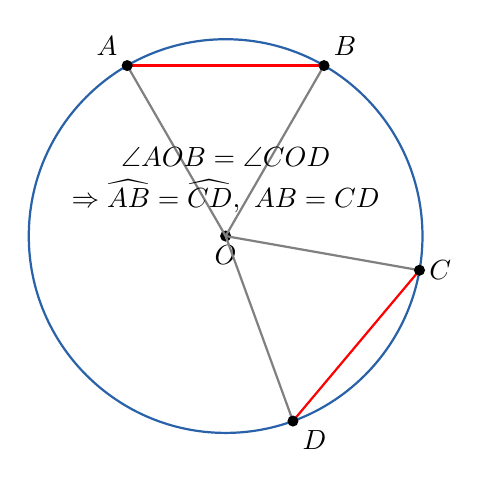
\begin{tikzpicture}[scale=1.0]
  \draw[thick, mainblue] (0,0) circle (2.5);
  \fill (0,0) circle (2pt) node[below]{$O$};
  % 两组等圆心角
  \coordinate (A) at ({2.5*cos(120)}, {2.5*sin(120)});
  \coordinate (B) at ({2.5*cos(60)}, {2.5*sin(60)});
  \coordinate (C) at ({2.5*cos(-10)}, {2.5*sin(-10)});
  \coordinate (D) at ({2.5*cos(-70)}, {2.5*sin(-70)});
  \draw[thick, red] (A) -- (B);
  \draw[thick, red] (C) -- (D);
  \draw[thick, gray] (0,0) -- (A);
  \draw[thick, gray] (0,0) -- (B);
  \draw[thick, gray] (0,0) -- (C);
  \draw[thick, gray] (0,0) -- (D);
  \fill (A) circle (2pt) node[above left]{$A$};
  \fill (B) circle (2pt) node[above right]{$B$};
  \fill (C) circle (2pt) node[right]{$C$};
  \fill (D) circle (2pt) node[below right]{$D$};
  % 标注
  \node at (0, 1.0) {$\angle AOB = \angle COD$};
  \node at (0, 0.5) {$\Rightarrow \widehat{AB} = \widehat{CD},\ AB = CD$};
\end{tikzpicture}
\end{center}

\begin{warnbox}[前提条件]
"等圆心角 $\Leftrightarrow$ 等弧 $\Leftrightarrow$ 等弦"必须在\textbf{同圆或等圆}中才成立。在不同大小的圆中，相等的圆心角所对的弧和弦不一定相等。
\end{warnbox}

% ==================== 24.4 圆周角定理 ====================
\subsection*{24.4\quad 圆周角定理}

\begin{knowledgebox}[圆周角定理]
\textbf{定理}：一条弧所对的圆周角等于它所对的圆心角的一半。

即：在 $\odot O$ 中，$\widehat{AB}$ 所对的圆心角为 $\angle AOB$，所对的圆周角为 $\angle ACB$（$C$ 在圆上），则
\[
\angle ACB = \frac{1}{2} \angle AOB
\]
\end{knowledgebox}

\begin{center}
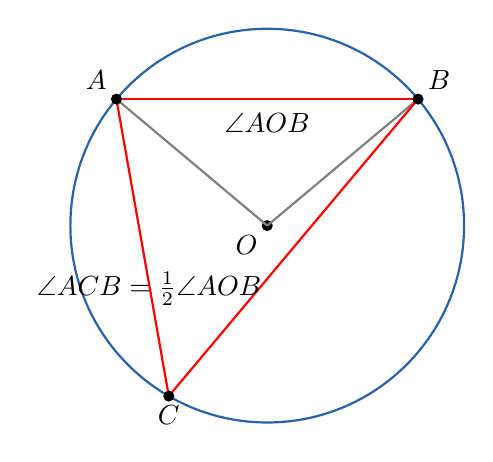
\begin{tikzpicture}[scale=1.0]
  \draw[thick, mainblue] (0,0) circle (2.5);
  \fill (0,0) circle (2pt) node[below left]{$O$};
  \coordinate (A) at ({-2.5*cos(40)}, {2.5*sin(40)});
  \coordinate (B) at ({2.5*cos(40)}, {2.5*sin(40)});
  \coordinate (C) at ({2.5*cos(-120)}, {2.5*sin(-120)});
  % 圆心角
  \draw[thick, gray] (0,0) -- (A);
  \draw[thick, gray] (0,0) -- (B);
  % 圆周角
  \draw[thick, red] (A) -- (C) -- (B);
  \draw[thick, red] (A) -- (B);
  \fill (A) circle (2pt) node[above left]{$A$};
  \fill (B) circle (2pt) node[above right]{$B$};
  \fill (C) circle (2pt) node[below]{$C$};
  % 标注
  \node at (0, 1.3) {$\angle AOB$};
  \node at (-1.5, -0.8) {$\angle ACB = \frac{1}{2}\angle AOB$};
\end{tikzpicture}
\end{center}

\begin{knowledgebox}[圆周角定理的推论]
\begin{enumerate}[nosep]
  \item \textbf{同弧上的圆周角相等}：在同圆或等圆中，同弧或等弧所对的圆周角相等。
  \item \textbf{半圆（直径）上的圆周角是直角}：半圆或直径所对的圆周角等于 $90°$。反之，$90°$ 的圆周角所对的弦是直径。
  \item \textbf{$90°$ 的圆周角所对的弦是直径}。
\end{enumerate}
\end{knowledgebox}

\begin{center}
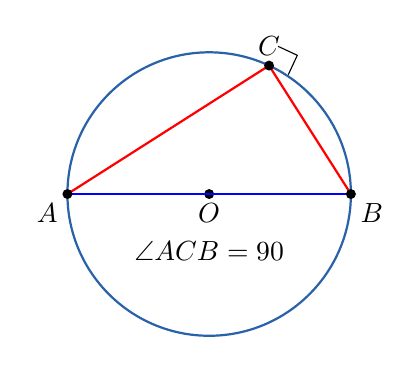
\begin{tikzpicture}[scale=0.9]
  % 半圆上的圆周角 = 90度
  \draw[thick, mainblue] (0,0) circle (2);
  \fill (0,0) circle (2pt) node[below]{$O$};
  \coordinate (A) at (-2, 0);
  \coordinate (B) at (2, 0);
  \coordinate (C) at ({2*cos(65)}, {2*sin(65)});
  \draw[thick, blue] (A) -- (B);
  \draw[thick, red] (A) -- (C) -- (B);
  \fill (A) circle (2pt) node[below left]{$A$};
  \fill (B) circle (2pt) node[below right]{$B$};
  \fill (C) circle (2pt) node[above]{$C$};
  % 直角标记
  \coordinate (P1) at ({2*cos(65)+0.3*cos(-25)}, {2*sin(65)+0.3*(-sin(25))});
  \coordinate (P2) at ({2*cos(65)+0.3*cos(-25)+0.3*cos(65)}, {2*sin(65)+0.3*(-sin(25))+0.3*sin(65)});
  \coordinate (P3) at ({2*cos(65)+0.3*cos(65)}, {2*sin(65)+0.3*sin(65)});
  \draw (P1) -- (P2) -- (P3);
  \node at (0, -0.8) {$\angle ACB = 90°$};
\end{tikzpicture}
\end{center}

\begin{warnbox}[易错提醒]
\begin{itemize}[nosep]
  \item 圆周角定理说的是"圆周角 $=$ 圆心角的\textbf{一半}"，不是相等。
  \item "同弧所对的圆周角相等"——注意是\textbf{同弧}或\textbf{等弧}，不是"同一条弦"。同一条弦所对的圆周角有两种情况（在弦的两侧），它们互补而非相等。
  \item "直径所对的圆周角 $= 90°$"的逆命题也成立：$90°$ 圆周角所对的弦是直径。这是证明"三点共圆"和"直角"的重要工具。
\end{itemize}
\end{warnbox}

% ==================== 24.5 圆内接四边形 ====================
\subsection*{24.5\quad 圆内接四边形}

\begin{knowledgebox}[圆内接四边形的性质]
\textbf{定理}：圆内接四边形的对角\textbf{互补}。

即：四边形 $ABCD$ 内接于 $\odot O$，则
\[
\angle A + \angle C = 180°, \quad \angle B + \angle D = 180°
\]
\end{knowledgebox}

\begin{center}
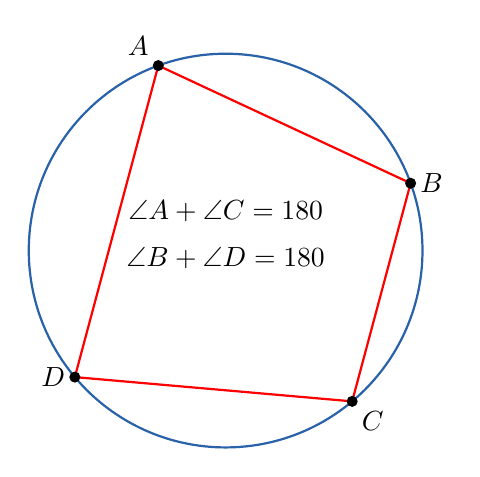
\begin{tikzpicture}[scale=1.0]
  \draw[thick, mainblue] (0,0) circle (2.5);
  \coordinate (A) at ({2.5*cos(110)}, {2.5*sin(110)});
  \coordinate (B) at ({2.5*cos(20)}, {2.5*sin(20)});
  \coordinate (C) at ({2.5*cos(-50)}, {2.5*sin(-50)});
  \coordinate (D) at ({2.5*cos(-140)}, {2.5*sin(-140)});
  \draw[thick, red] (A) -- (B) -- (C) -- (D) -- cycle;
  \fill (A) circle (2pt) node[above left]{$A$};
  \fill (B) circle (2pt) node[right]{$B$};
  \fill (C) circle (2pt) node[below right]{$C$};
  \fill (D) circle (2pt) node[left]{$D$};
  \node at (0, 0.5) {$\angle A + \angle C = 180°$};
  \node at (0, -0.1) {$\angle B + \angle D = 180°$};
\end{tikzpicture}
\end{center}

\begin{knowledgebox}[圆内接四边形的判定]
如果一个四边形的一组对角互补，那么这个四边形内接于圆（即四个顶点共圆）。
\end{knowledgebox}

\begin{tipbox}[圆内接四边形的外角]
圆内接四边形的一个外角等于它的内对角。即：$\angle DCE = \angle A$（其中 $\angle DCE$ 是 $\angle BCD$ 的外角）。
\end{tipbox}

% ==================== 24.6 点与圆的位置关系 ====================
\subsection*{24.6\quad 点与圆的位置关系}

\begin{knowledgebox}[点与圆的位置关系]
设 $\odot O$ 的半径为 $r$，点 $P$ 到圆心 $O$ 的距离为 $d = |OP|$，则：
\begin{center}
\begin{tabular}{c|c|c}
\toprule
位置关系 & 条件 & 图示描述 \\
\midrule
点在圆\textbf{外} & $d > r$ & 点在圆外 \\
点在圆\textbf{上} & $d = r$ & 点在圆周上 \\
点在圆\textbf{内} & $d < r$ & 点在圆内 \\
\bottomrule
\end{tabular}
\end{center}
\end{knowledgebox}

\begin{center}
\begin{tikzpicture}[scale=0.9]
  \draw[thick, mainblue] (0,0) circle (2);
  \fill (0,0) circle (2pt) node[below left]{$O$};
  % 点在圆外
  \coordinate (P1) at (3, 1);
  \fill (P1) circle (2pt) node[right]{$P_1$（圆外，$d > r$）};
  \draw[dashed, gray] (0,0) -- (P1);
  % 点在圆上
  \coordinate (P2) at ({2*cos(30)}, {2*sin(30)});
  \fill (P2) circle (2pt) node[above right]{$P_2$（圆上，$d = r$）};
  % 点在圆内
  \coordinate (P3) at (-0.8, -0.5);
  \fill (P3) circle (2pt) node[below left]{$P_3$（圆内，$d < r$）};
  \draw[dashed, gray] (0,0) -- (P3);
\end{tikzpicture}
\end{center}

% ==================== 24.7 直线与圆的位置关系 ====================
\subsection*{24.7\quad 直线与圆的位置关系}

\begin{knowledgebox}[直线与圆的三种位置关系]
设 $\odot O$ 的半径为 $r$，圆心 $O$ 到直线 $l$ 的距离为 $d$，则：

\begin{center}
\begin{tabular}{c|c|c}
\toprule
位置关系 & 条件 & 交点个数 \\
\midrule
\textbf{相离}（直线与圆无交点） & $d > r$ & $0$ 个 \\
\textbf{相切}（直线与圆有一个交点） & $d = r$ & $1$ 个 \\
\textbf{相交}（直线与圆有两个交点） & $d < r$ & $2$ 个 \\
\bottomrule
\end{tabular}
\end{center}
\end{knowledgebox}

\begin{center}
\begin{tikzpicture}[scale=0.8]
  % 相离
  \begin{scope}[shift={(-4,0)}]
    \draw[thick, mainblue] (0,0) circle (1.5);
    \draw[thick, red] (-2.5, 2.2) -- (2.5, 2.2);
    \draw[dashed, gray] (0,0) -- (0, 2.2);
    \node[below, font=\small] at (0, -2) {相离 $d > r$};
    \node[left, font=\small, gray] at (0, 1.1) {$d$};
  \end{scope}
  % 相切
  \begin{scope}[shift={(0,0)}]
    \draw[thick, mainblue] (0,0) circle (1.5);
    \draw[thick, red] (-2.5, 1.5) -- (2.5, 1.5);
    \draw[dashed, gray] (0,0) -- (0, 1.5);
    \fill (0, 1.5) circle (2pt);
    \node[below, font=\small] at (0, -2) {相切 $d = r$};
  \end{scope}
  % 相交
  \begin{scope}[shift={(4,0)}]
    \draw[thick, mainblue] (0,0) circle (1.5);
    \draw[thick, red] (-2.5, 0.5) -- (2.5, 0.5);
    \draw[dashed, gray] (0,0) -- (0, 0.5);
    \fill ({-sqrt(1.5*1.5-0.5*0.5)}, 0.5) circle (2pt);
    \fill ({sqrt(1.5*1.5-0.5*0.5)}, 0.5) circle (2pt);
    \node[below, font=\small] at (0, -2) {相交 $d < r$};
  \end{scope}
\end{tikzpicture}
\end{center}

% ==================== 24.8 切线的性质和判定 ====================
\subsection*{24.8\quad 切线的性质和判定}

\begin{knowledgebox}[切线的定义]
\textbf{切线}：与圆只有一个公共点的直线叫做圆的切线。这个公共点叫做\textbf{切点}。

\textbf{割线}：与圆有两个公共点的直线叫做圆的割线。
\end{knowledgebox}

\begin{knowledgebox}[切线的性质]
\textbf{性质1}：圆的切线垂直于过切点的半径。

即：若直线 $l$ 切 $\odot O$ 于点 $A$，则 $l \perp OA$。

\textbf{性质2}：经过圆心且垂直于切线的直线必经过切点。

\textbf{性质3}：经过切点且垂直于切线的直线必经过圆心。
\end{knowledgebox}

\begin{center}
\begin{tikzpicture}[scale=1.0]
  \draw[thick, mainblue] (0,0) circle (2);
  \fill (0,0) circle (2pt) node[below left]{$O$};
  \coordinate (A) at (2, 0);
  \draw[thick, red] (A) -- ++(0, 2.5) -- ++(0, -5);
  \fill (A) circle (2pt) node[below right]{$A$（切点）};
  \draw[thick, blue] (0,0) -- (A);
  % 垂直标记
  \draw (1.65, 0) -- (1.65, 0.35) -- (2, 0.35);
  \node[above, red] at (2, 2.2) {$l$（切线）};
  \node[above, blue] at (1, 0.15) {$OA \perp l$};
\end{tikzpicture}
\end{center}

\begin{knowledgebox}[切线的判定]
\textbf{判定方法}：

\begin{enumerate}[nosep]
  \item \textbf{定义法}：与圆只有一个公共点的直线是切线。
  \item \textbf{距离法}：到圆心的距离等于半径的直线是切线。即若 $d(O,\, l) = r$，则 $l$ 是切线。
  \item \textbf{判定定理}：经过半径的外端并且垂直于这条半径的直线是圆的切线。
\end{enumerate}
\end{knowledgebox}

\begin{tipbox}[证明切线的两种常见情况]
\begin{enumerate}[nosep]
  \item \textbf{已知交点在圆上}（即已知切点）：连圆心和该点，证垂直。"连半径，证垂直"。
  \item \textbf{未知交点是否在圆上}：过圆心作直线的垂线，证垂线段长等于半径。"作垂直，证等半径"。
\end{enumerate}
\end{tipbox}

% ==================== 24.9 切线长定理 ====================
\subsection*{24.9\quad 切线长定理}

\begin{knowledgebox}[切线长]
\textbf{切线长}：过圆外一点 $P$ 作圆的切线，切点为 $A$，线段 $PA$ 的长叫做点 $P$ 到圆的\textbf{切线长}。
\end{knowledgebox}

\begin{knowledgebox}[切线长定理]
\textbf{定理}：从圆外一点引圆的两条切线，它们的切线长相等，圆心和这一点的连线平分两条切线的夹角。

即：$PA$、$PB$ 是 $\odot O$ 的两条切线，$A$、$B$ 为切点，则：
\[
PA = PB, \quad \angle OPA = \angle OPB, \quad OA \perp PA, \quad OB \perp PB
\]
\end{knowledgebox}

\begin{center}
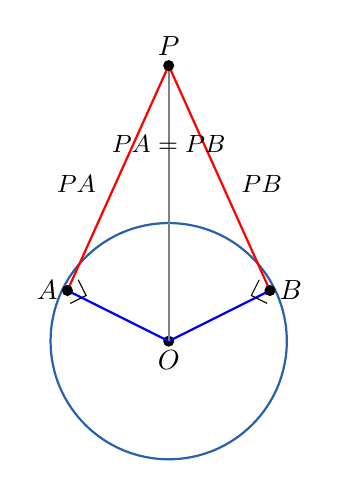
\begin{tikzpicture}[scale=1.0]
  \draw[thick, mainblue] (0,0) circle (1.5);
  \fill (0,0) circle (2pt) node[below]{$O$};
  \coordinate (P) at (0, 3.5);
  \coordinate (A) at ({-1.5*3.5/sqrt(3.5*3.5-1.5*1.5)*sqrt(1-1.5*1.5/(3.5*3.5))}, {1.5*1.5/3.5});
  \coordinate (B) at ({1.5*3.5/sqrt(3.5*3.5-1.5*1.5)*sqrt(1-1.5*1.5/(3.5*3.5))}, {1.5*1.5/3.5});
  % 简化计算：P = (0, 3.5), r = 1.5, 切点坐标
  \coordinate (A) at (-1.286, 0.643);
  \coordinate (B) at (1.286, 0.643);
  \draw[thick, red] (P) -- (A);
  \draw[thick, red] (P) -- (B);
  \draw[thick, blue] (0,0) -- (A);
  \draw[thick, blue] (0,0) -- (B);
  \draw[thick, gray] (0,0) -- (P);
  \fill (P) circle (2pt) node[above]{$P$};
  \fill (A) circle (2pt) node[left]{$A$};
  \fill (B) circle (2pt) node[right]{$B$};
  % 垂直标记
  \draw (-1.15, 0.78) -- (-1.05, 0.58) -- (-1.25, 0.48);
  \draw (1.15, 0.78) -- (1.05, 0.58) -- (1.25, 0.48);
  % 等长标记
  \node[left, font=\small] at (-0.8, 2) {$PA$};
  \node[right, font=\small] at (0.8, 2) {$PB$};
  \node[font=\small] at (0, 2.5) {$PA = PB$};
\end{tikzpicture}
\end{center}

\begin{tipbox}[切线长定理的几何意义]
切线长定理的结论可以概括为"三个一"：
\begin{itemize}[nosep]
  \item \textbf{一切线长}相等：$PA = PB$；
  \item \textbf{一角}被平分：$OP$ 平分 $\angle APB$；
  \item \textbf{一垂直}：$OA \perp PA$，$OB \perp PB$。
\end{itemize}
\end{tipbox}

% ==================== 24.10 弧长与扇形面积 ====================
\subsection*{24.10\quad 弧长公式与扇形面积公式}

\begin{knowledgebox}[弧长公式]
半径为 $r$ 的圆中，$n°$ 的圆心角所对的弧长为：
\[
l = \frac{n\pi r}{180}
\]
其中 $n$ 为圆心角的度数，$r$ 为半径。
\end{knowledgebox}

\begin{knowledgebox}[扇形面积公式]
由圆心角的两条半径和圆心角所对的弧围成的图形叫做\textbf{扇形}。

扇形面积公式：
\[
S = \frac{n\pi r^2}{360} = \frac{1}{2}lr
\]
其中 $n$ 为圆心角的度数，$r$ 为半径，$l$ 为弧长。
\end{knowledgebox}

\begin{center}
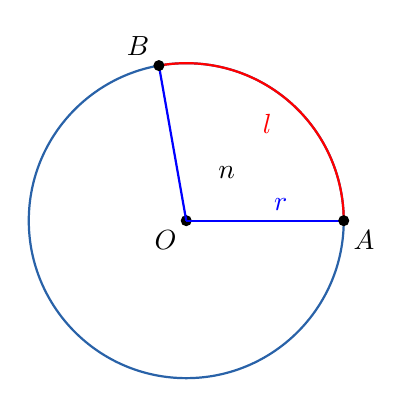
\begin{tikzpicture}[scale=1.0]
  \draw[thick, mainblue] (0,0) circle (2);
  \fill (0,0) circle (2pt) node[below left]{$O$};
  \coordinate (A) at (2, 0);
  \coordinate (B) at ({2*cos(100)}, {2*sin(100)});
  \draw[thick, blue] (0,0) -- (A);
  \draw[thick, blue] (0,0) -- (B);
  % 弧
  \draw[thick, red] (A) arc (0:100:2);
  \fill (A) circle (2pt) node[below right]{$A$};
  \fill (B) circle (2pt) node[above left]{$B$};
  % 标注
  \node at ({0.8*cos(50)}, {0.8*sin(50)}) {$n°$};
  \node[red] at ({1.6*cos(50)}, {1.6*sin(50)}) {$l$};
  \node[blue] at (1.2, 0.2) {$r$};
\end{tikzpicture}
\end{center}

\begin{warnbox}[公式使用注意]
\begin{itemize}[nosep]
  \item 弧长公式中 $n$ 是\textbf{角度}不是弧度，不要与弧度制混淆。
  \item 扇形面积的两个公式：已知圆心角用 $S = \dfrac{n\pi r^2}{360}$，已知弧长用 $S = \dfrac{1}{2}lr$。
  \item 扇形面积与弧长的关系：$S = \dfrac{1}{2}lr$，形式上类似于三角形面积 $S = \dfrac{1}{2} \times$ 底 $\times$ 高。
\end{itemize}
\end{warnbox}

% ==================== 24.11 正多边形与圆 ====================
\subsection*{24.11\quad 正多边形与圆}

\begin{knowledgebox}[正多边形与圆的关系]
\begin{enumerate}[nosep]
  \item 把圆分成 $n$（$n \geq 3$）等份，依次连接各分点所得的多边形是圆的\textbf{内接正 $n$ 边形}。
  \item 正多边形的外接圆的圆心叫做正多边形的\textbf{中心}。
  \item 外接圆的半径叫做正多边形的\textbf{半径}。
  \item 中心到正多边形一边的距离叫做正多边形的\textbf{边心距}。
\end{enumerate}
\end{knowledgebox}

\begin{knowledgebox}[正 $n$ 边形的计算公式]
设正 $n$ 边形的半径为 $R$，边心距为 $r$，边长为 $a$，则：
\begin{enumerate}[nosep]
  \item 每个内角 $= \dfrac{(n-2) \times 180°}{n}$。
  \item 每个中心角 $= \dfrac{360°}{n}$。
  \item 边长 $a = 2R\sin\dfrac{180°}{n}$。
  \item 边心距 $r = R\cos\dfrac{180°}{n}$。
  \item 周长 $P = na$。
  \item 面积 $S = \dfrac{1}{2} \times$ 周长 $\times$ 边心距 $= \dfrac{1}{2}Pr = \dfrac{1}{2}nar$。
\end{enumerate}
\end{knowledgebox}

\begin{center}
\begin{tikzpicture}[scale=1.2]
  % 正六边形
  \draw[thick, mainblue] (0,0) circle (2);
  \foreach \i in {0,1,2,3,4,5} {
    \coordinate (V\i) at ({2*cos(90+\i*60)}, {2*sin(90+\i*60)});
  }
  \draw[thick, red] (V0) -- (V1) -- (V2) -- (V3) -- (V4) -- (V5) -- cycle;
  \fill (0,0) circle (2pt) node[below left]{$O$};
  % 半径
  \draw[thick, blue] (0,0) -- (V0);
  \node[blue, above right] at (0.3, 1.2) {$R$};
  % 边心距
  \coordinate (M) at ({(V0)+(V1)});  % 中点
  \draw[dashed, gray] (0,0) -- ({cos(90+30)}, {sin(90+30)});
  \node[gray, right] at (0.55, 0.85) {$r$};
  % 标注边长
  \node[red, above right] at ({0.5*(V0)+(0.5)*(V1)}) {$a$};
  % 中心角
  \draw[->, thick, tipgreen] (0.5, 0) arc (0:60:0.5);
  \node[tipgreen] at (0.45, 0.35) {$60°$};
  \node[below] at (0, -2.5) {正六边形};
\end{tikzpicture}
\end{center}

% ==================== 24.12 圆锥的侧面积和全面积 ====================
\subsection*{24.12\quad 圆锥的侧面积和全面积}

\begin{knowledgebox}[圆锥的相关概念]
\begin{itemize}[nosep]
  \item \textbf{圆锥的底面}：圆锥底面是一个圆。
  \item \textbf{圆锥的母线}：连接圆锥顶点和底面圆周上任意一点的线段。所有母线长相等。
  \item \textbf{圆锥的高}：从顶点到底面圆心的距离。
  \item \textbf{侧面展开图}：圆锥的侧面展开图是一个\textbf{扇形}，扇形的半径等于母线长 $l$，扇形的弧长等于底面圆的周长 $2\pi r$。
\end{itemize}
\end{knowledgebox}

\begin{knowledgebox}[圆锥的侧面积和全面积]
设圆锥的底面半径为 $r$，母线长为 $l$，则：
\begin{enumerate}[nosep]
  \item \textbf{侧面积}：$S_{\text{侧}} = \pi r l$
  \item \textbf{底面积}：$S_{\text{底}} = \pi r^2$
  \item \textbf{全面积}：$S_{\text{全}} = S_{\text{侧}} + S_{\text{底}} = \pi r l + \pi r^2 = \pi r(l + r)$
\end{enumerate}

其中母线 $l$、高 $h$、底面半径 $r$ 满足：$l^2 = h^2 + r^2$（由勾股定理）。
\end{knowledgebox}

\begin{center}
\begin{tikzpicture}[scale=0.9]
  % 左侧：圆锥
  \begin{scope}[shift={(-3,0)}]
    \draw[thick, mainblue] (0,0) ellipse (1.5 and 0.5);
    \draw[thick, mainblue] (-1.5,0) -- (0,3) -- (1.5,0);
    \draw[dashed, gray] (0,0) -- (0,3);
    \draw[dashed, gray] (0,0) -- (1.5,0);
    \fill (0,3) circle (2pt) node[above]{$V$};
    \fill (0,0) circle (2pt) node[below]{$O$};
    \node[right, font=\small] at (0.8, 1.5) {$l$（母线）};
    \node[below, font=\small] at (0.75, -0.1) {$r$};
    \node[left, font=\small] at (-0.3, 1.5) {$h$};
    \node[below] at (0, -1) {圆锥};
  \end{scope}
  % 右侧：侧面展开图
  \begin{scope}[shift={(3,0)}]
    \draw[thick, red] (0,0) -- (2.5, 0) arc (0:108:2.5) -- cycle;
    \fill (0,0) circle (2pt) node[below left]{$V$};
    \node[right, font=\small] at (1.5, 1) {$l$};
    \node[above, font=\small] at (1.25, 0) {$\widehat{AB}$};
    \node[below] at (1, -0.5) {侧面展开图（扇形）};
  \end{scope}
\end{tikzpicture}
\end{center}

\begin{tipbox}[侧面展开图的圆心角]
设侧面展开图扇形的圆心角为 $\theta$，则：
\[
\theta = \frac{r}{l} \times 360° = \frac{2\pi r}{2\pi l} \times 360°
\]
即：扇形弧长 $=$ 底面圆周长，$l\theta_{\text{rad}} = 2\pi r$。
\end{tipbox}

% ==============================================================
% 第二部分：例题精讲
% ==============================================================
\section*{\textcolor{examorange}{二、例题精讲}}

\begin{examplebox}[【例题1】垂径定理的基本应用]
在 $\odot O$ 中，弦 $AB = 8$，圆心 $O$ 到弦 $AB$ 的距离（弦心距）为 $3$，求圆的半径。
\end{examplebox}

\textbf{解：}

设 $M$ 为 $AB$ 的中点，连接 $OM$，则 $OM \perp AB$（垂径定理）。

$AM = \dfrac{AB}{2} = \dfrac{8}{2} = 4$，$OM = 3$。

在直角三角形 $OMA$ 中，由勾股定理：
\[
OA = \sqrt{OM^2 + AM^2} = \sqrt{9 + 16} = \sqrt{25} = 5
\]

所以圆的半径为 $\boxed{5}$。

\begin{tipbox}[方法总结]
垂径定理与勾股定理的结合是圆中最基本的计算题型。关键是过圆心作弦的垂线，构成直角三角形，利用 $r^2 = d^2 + \left(\dfrac{l}{2}\right)^2$ 求解。
\end{tipbox}

\vspace{6pt}

\begin{examplebox}[【例题2】圆周角定理的应用]
如图，$AB$ 是 $\odot O$ 的直径，$C$、$D$ 是圆上的点，$\angle BAC = 30°$。求 $\angle ADC$ 的度数。
\end{examplebox}

\textbf{解：}

因为 $AB$ 是直径，所以 $\angle ACB = 90°$（直径所对的圆周角为 $90°$）。

在 $\triangle ABC$ 中：
\[
\angle ABC = 180° - 90° - 30° = 60°
\]

因为 $\angle ADC$ 和 $\angle ABC$ 都是弧 $\widehat{AC}$ 所对的圆周角（在同弧上），所以：
\[
\angle ADC = \angle ABC = 60°
\]

\begin{tipbox}[方法总结]
圆周角定理的核心应用：
\begin{itemize}[nosep]
  \item 直径所对的圆周角 $= 90°$。
  \item 同弧上的圆周角相等。
  \item 圆周角 $= \dfrac{1}{2}$ 圆心角。
\end{itemize}
解题时先识别"直径""同弧""半圆"等关键条件。
\end{tipbox}

\vspace{6pt}

\begin{examplebox}[【例题3】圆内接四边形的性质应用]
四边形 $ABCD$ 内接于 $\odot O$，$\angle A = 75°$，$\angle B = 110°$。求 $\angle C$ 和 $\angle D$ 的度数。
\end{examplebox}

\textbf{解：}

由圆内接四边形对角互补：
\[
\angle A + \angle C = 180° \implies \angle C = 180° - 75° = 105°
\]
\[
\angle B + \angle D = 180° \implies \angle D = 180° - 110° = 70°
\]

验证：四边形内角和 $= 75° + 110° + 105° + 70° = 360°$，正确。

\begin{tipbox}[方法总结]
圆内接四边形的对角互补，利用这一性质可以直接求角。注意"对角"指的是不相邻的两个角（$\angle A$ 与 $\angle C$，$\angle B$ 与 $\angle D$）。
\end{tipbox}

\vspace{6pt}

\begin{examplebox}[【例题4】证明题——切线的判定]
如图，$AB$ 是 $\odot O$ 的直径，$C$ 是圆上一点，$CD \perp AB$ 于 $D$，$CE$ 是 $\angle ACB$ 的平分线。求证：$CE$ 是 $\odot O$ 的切线。

\begin{center}
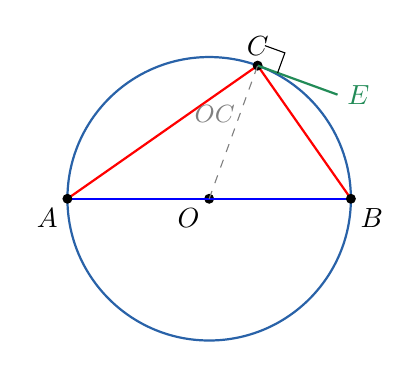
\begin{tikzpicture}[scale=0.9]
  \draw[thick, mainblue] (0,0) circle (2);
  \fill (0,0) circle (2pt) node[below left]{$O$};
  \coordinate (A) at (-2, 0);
  \coordinate (B) at (2, 0);
  \coordinate (C) at ({2*cos(70)}, {2*sin(70)});
  \draw[thick, blue] (A) -- (B);
  \draw[thick, red] (A) -- (C) -- (B);
  \fill (A) circle (2pt) node[below left]{$A$};
  \fill (B) circle (2pt) node[below right]{$B$};
  \fill (C) circle (2pt) node[above]{$C$};
  % CE (切线方向)
  \coordinate (E) at ({2*cos(70)+1.2*cos(-20)}, {2*sin(70)+1.2*sin(-20)});
  \draw[thick, tipgreen] (C) -- (E);
  \node[right, tipgreen] at (E) {$E$};
  % OC
  \draw[dashed, gray] (0,0) -- (C);
  \node[left, gray, font=\small] at (0.5, 1.2) {$OC$};
  % 直角标记
  \coordinate (P1) at ({2*cos(70)+0.3*cos(-20)}, {2*sin(70)+0.3*sin(-20)});
  \coordinate (P2) at ({2*cos(70)+0.3*cos(-20)+0.3*cos(70)}, {2*sin(70)+0.3*sin(-20)+0.3*sin(70)});
  \coordinate (P3) at ({2*cos(70)+0.3*cos(70)}, {2*sin(70)+0.3*sin(70)});
  \draw (P1) -- (P2) -- (P3);
\end{tikzpicture}
\end{center}
\end{examplebox}

\textbf{证明：}

连接 $OC$。

因为 $OC = OA$（都是半径），所以 $\triangle OAC$ 是等腰三角形，$\angle OCA = \angle OAC$。

因为 $AB$ 是直径，所以 $\angle ACB = 90°$（直径所对的圆周角为直角）。

因为 $CE$ 平分 $\angle ACB$，所以 $\angle ACE = \angle BCE = 45°$。

因此 $\angle OCE = \angle OCA + \angle ACE = \angle OAC + 45°$。

在 $\triangle ACB$ 中，$\angle CAB + \angle CBA = 90°$。

又 $\angle OAC = \angle CAB$，所以 $\angle OCE = \angle CAB + 45°$。

另一方面，$\angle OCA + \angle ACE = \angle CAB + 45°$。

我们需要证明 $CE \perp OC$，即 $\angle OCE = 90°$。

由 $\angle OCA = \angle CAB$ 和 $\angle ACE = 45°$：
\[
\angle OCE = \angle OCA + \angle ACE = \angle CAB + 45°
\]

在直角三角形 $ACB$ 中，设 $\angle CAB = \alpha$，则 $\angle CBA = 90° - \alpha$。
因为 $OC = OB$，$\angle OCB = \angle OBC = 90° - \alpha$。
所以 $\angle OCA = \alpha$。

$\angle OCE = \alpha + 45°$。

我们需要 $\alpha + 45° = 90°$，即 $\alpha = 45°$。

但这不一定成立。让我重新审视此题。

\textbf{修正}：此题需要 $C$ 在特定位置。让我换一个更标准的切线判定题。

\begin{examplebox}[【例题4】证明题——切线的判定（修正）]
如图，$AB$ 是 $\odot O$ 的直径，$C$ 是 $\odot O$ 上一点，过 $C$ 作直线 $l$，使得 $OC \perp l$。求证：$l$ 是 $\odot O$ 的切线。
\end{examplebox}

\textbf{证明：}

因为 $OC$ 是 $\odot O$ 的半径，$l$ 过点 $C$ 且 $OC \perp l$。

由切线的判定定理：\textbf{经过半径的外端并且垂直于这条半径的直线是圆的切线}。

因为 $C$ 在 $\odot O$ 上（即 $C$ 是半径 $OC$ 的外端），且 $l \perp OC$，所以 $l$ 是 $\odot O$ 的切线。

\begin{tipbox}[方法总结]
证明切线的标准方法：
\begin{enumerate}[nosep]
  \item 若已知直线与圆有交点 $C$："连半径 $OC$，证 $OC \perp l$"。
  \item 若未知交点位置："作 $OH \perp l$ 于 $H$，证 $OH = r$"。
\end{enumerate}
本题是直接用判定定理，属于最简单的切线判定。
\end{tipbox}

\vspace{6pt}

\begin{examplebox}[【例题5】切线长定理的综合应用]
如图，$PA$、$PB$ 是 $\odot O$ 的两条切线，$A$、$B$ 为切点，$\angle APB = 60°$，$\odot O$ 的半径为 $3$。求 $PA$ 的长和四边形 $PAOB$ 的面积。

\begin{center}
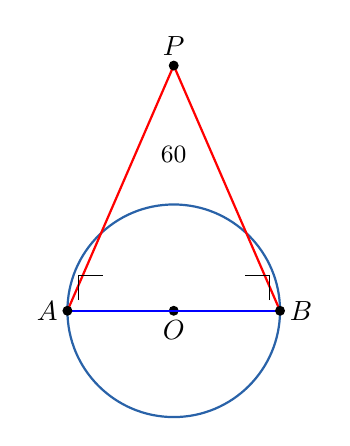
\begin{tikzpicture}[scale=0.9]
  \draw[thick, mainblue] (0,0) circle (1.5);
  \fill (0,0) circle (2pt) node[below]{$O$};
  \coordinate (P) at (0, 3.46);
  \coordinate (A) at (-1.5, 0);
  \coordinate (B) at (1.5, 0);
  \draw[thick, red] (P) -- (A);
  \draw[thick, red] (P) -- (B);
  \draw[thick, blue] (0,0) -- (A);
  \draw[thick, blue] (0,0) -- (B);
  \fill (P) circle (2pt) node[above]{$P$};
  \fill (A) circle (2pt) node[left]{$A$};
  \fill (B) circle (2pt) node[right]{$B$};
  % 垂直标记
  \draw (-1.35, 0.15) -- (-1.35, 0.5) -- (-1.0, 0.5);
  \draw (1.35, 0.15) -- (1.35, 0.5) -- (1.0, 0.5);
  \node[font=\small] at (0, 2.2) {$60°$};
\end{tikzpicture}
\end{center}
\end{examplebox}

\textbf{解：}

连接 $OA$，$OB$，$OP$。

由切线长定理：$PA = PB$，$OP$ 平分 $\angle APB$，$OA \perp PA$，$OB \perp PB$。

所以 $\angle OPA = \dfrac{1}{2} \times 60° = 30°$。

在直角三角形 $OAP$ 中，$\angle OAP = 90°$，$\angle OPA = 30°$，$OA = 3$：
\[
PA = \frac{OA}{\tan 30°} = \frac{3}{\frac{\sqrt{3}}{3}} = \frac{3 \times 3}{\sqrt{3}} = 3\sqrt{3}
\]

四边形 $PAOB$ 的面积 $= 2 \times S_{\triangle OAP}$：
\[
S_{\triangle OAP} = \frac{1}{2} \times OA \times PA = \frac{1}{2} \times 3 \times 3\sqrt{3} = \frac{9\sqrt{3}}{2}
\]
\[
S_{PAOB} = 2 \times \frac{9\sqrt{3}}{2} = 9\sqrt{3}
\]

\begin{tipbox}[方法总结]
切线长定理问题的一般步骤：连圆心与切点（得到垂直关系），连圆心与圆外点（得到角平分线），在直角三角形中用三角函数或勾股定理求解。
\end{tipbox}

\vspace{6pt}

\begin{examplebox}[【例题6】弧长与扇形面积计算]
一个扇形的圆心角为 $120°$，半径为 $6$ cm，求：
\begin{enumerate}[label=(\arabic*)]
  \item 扇形的弧长。
  \item 扇形的面积。
\end{enumerate}
\end{examplebox}

\textbf{解：}
\begin{enumerate}[label=(\arabic*)]
  \item 弧长：
  \[
  l = \frac{n\pi r}{180} = \frac{120 \times \pi \times 6}{180} = \frac{720\pi}{180} = 4\pi \text{（cm）}
  \]
  \item 扇形面积：
  \[
  S = \frac{n\pi r^2}{360} = \frac{120 \times \pi \times 36}{360} = \frac{4320\pi}{360} = 12\pi \text{（cm}^2\text{）}
  \]
  验证：$S = \dfrac{1}{2}lr = \dfrac{1}{2} \times 4\pi \times 6 = 12\pi$，一致。
\end{enumerate}

\begin{tipbox}[方法总结]
弧长和扇形面积公式中，$n$ 都是圆心角的\textbf{度数}。记忆技巧：弧长是圆周长的 $\dfrac{n}{360}$，扇形面积是圆面积的 $\dfrac{n}{360}$。
\end{tipbox}

\vspace{6pt}

\begin{examplebox}[【例题7】圆锥的侧面积计算]
一个圆锥的底面半径为 $3$ cm，母线长为 $5$ cm，求：
\begin{enumerate}[label=(\arabic*)]
  \item 圆锥的侧面积。
  \item 圆锥的全面积。
  \item 侧面展开图的圆心角。
\end{enumerate}
\end{examplebox}

\textbf{解：}

$r = 3$，$l = 5$。
\begin{enumerate}[label=(\arabic*)]
  \item 侧面积：
  \[
  S_{\text{侧}} = \pi r l = \pi \times 3 \times 5 = 15\pi \text{（cm}^2\text{）}
  \]
  \item 全面积：
  \[
  S_{\text{全}} = \pi r l + \pi r^2 = 15\pi + 9\pi = 24\pi \text{（cm}^2\text{）}
  \]
  \item 侧面展开图的圆心角：
  \[
  \theta = \frac{r}{l} \times 360° = \frac{3}{5} \times 360° = 216°
  \]
\end{enumerate}

\begin{tipbox}[方法总结]
圆锥问题的核心关系：
\begin{itemize}[nosep]
  \item 展开图的扇形弧长 $=$ 底面圆周长 $= 2\pi r$。
  \item 展开图的扇形半径 $=$ 母线长 $= l$。
  \item 圆锥的高、底面半径、母线构成直角三角形：$l^2 = h^2 + r^2$。
\end{itemize}
\end{tipbox}

\vspace{6pt}

\begin{examplebox}[【例题8】综合题——垂径定理与勾股定理]
在 $\odot O$ 中，直径 $AB = 10$，弦 $CD = 8$，$AB \parallel CD$。求弦 $AB$ 与弦 $CD$ 之间的距离。
\end{examplebox}

\textbf{解：}

设 $M$ 为 $AB$ 的中点（即圆心 $O$），$N$ 为 $CD$ 的中点。

连接 $ON$，则 $ON \perp CD$（垂径定理推论：平分弦的直径垂直于弦）。

$OC = 5$（半径），$CN = \dfrac{CD}{2} = 4$。

在直角三角形 $ONC$ 中：
\[
ON = \sqrt{OC^2 - CN^2} = \sqrt{25 - 16} = \sqrt{9} = 3
\]

因为 $AB \parallel CD$，所以 $AB$ 与 $CD$ 之间的距离 $= ON = 3$。

注意：$CD$ 可能在 $AB$ 的上方或下方，所以距离为 $3$（取正值）。

\begin{warnbox}[注意]
\begin{itemize}[nosep]
  \item 平行弦之间的距离需要考虑两种情况：弦在圆心同侧或异侧。本题中 $AB$ 是直径（经过圆心），所以只有一种情况。
  \item 如果两条平行弦都不是直径，需要讨论它们在圆心同侧和异侧两种情况。
\end{itemize}
\end{warnbox}

\vspace{6pt}

\begin{examplebox}[【例题9】综合提高——正多边形的面积]
求边长为 $6$ 的正六边形的面积。
\end{examplebox}

\textbf{解：}

正六边形可以分成 $6$ 个等边三角形，每个等边三角形的边长为 $6$。

一个边长为 $a$ 的等边三角形面积 $= \dfrac{\sqrt{3}}{4}a^2$。

所以每个小三角形面积 $= \dfrac{\sqrt{3}}{4} \times 36 = 9\sqrt{3}$。

正六边形面积 $= 6 \times 9\sqrt{3} = 54\sqrt{3}$。

\begin{tipbox}[方法总结]
正多边形面积的求法：
\begin{itemize}[nosep]
  \item 正 $n$ 边形可以分成 $n$ 个全等的等腰三角形，每个三角形的顶点在中心。
  \item 面积 $= \dfrac{1}{2} \times$ 周长 $\times$ 边心距。
  \item 正六边形特殊：可分成 $6$ 个等边三角形。
\end{itemize}
\end{tipbox}

% ==============================================================
% 第三部分：应用题
% ==============================================================
\section*{\textcolor{apppurple}{三、应用题}}

\begin{appbox}[【应用1】拱桥问题]
一座圆弧形拱桥的跨度为 $20$ 米，拱高为 $4$ 米。求拱桥所在圆的半径。

\begin{center}
\begin{tikzpicture}[scale=0.6]
  \draw[thick, mainblue] (0,0) arc (180:0:7.2);
  \draw[thick, gray] (-7.2, 0) -- (7.2, 0);
  \fill (-7.2, 0) circle (3pt) node[below]{$A$};
  \fill (7.2, 0) circle (3pt) node[below]{$B$};
  \fill (0, 3) circle (3pt) node[above]{$C$};
  \draw[dashed, gray] (0,0) -- (0, 3);
  \node[right, font=\small] at (0.3, 1.5) {$4$ m};
  \node[below, font=\small] at (0, -0.3) {$20$ m};
  % 圆心
  \fill (0, -5.04) circle (2pt) node[below]{$O$};
  \draw[dashed, gray] (0, -5.04) -- (0, 3);
  \draw[dashed, gray] (0, -5.04) -- (7.2, 0);
\end{tikzpicture}
\end{center}
\end{appbox}

\textbf{解：}

设拱桥所在圆的圆心为 $O$，半径为 $R$。

设 $AB$ 的中点为 $M$，则 $M$ 为拱顶。$AB = 20$，$CM = 4$（拱高）。

由垂径定理，$OM \perp AB$，$AM = 10$。

$OC = R$，$OM = R - 4$。

在直角三角形 $OMA$ 中：
\[
OA^2 = OM^2 + AM^2
\]
\[
R^2 = (R - 4)^2 + 10^2
\]
\[
R^2 = R^2 - 8R + 16 + 100
\]
\[
8R = 116 \implies R = 14.5
\]

拱桥所在圆的半径为 $\boxed{14.5}$ 米。

\vspace{6pt}

\begin{appbox}[【应用2】管道截面问题]
一段圆形排水管道的内径（直径）为 $60$ cm，管内积水的最大深度为 $20$ cm（水面到管底的距离）。求水面的宽度。

\begin{center}
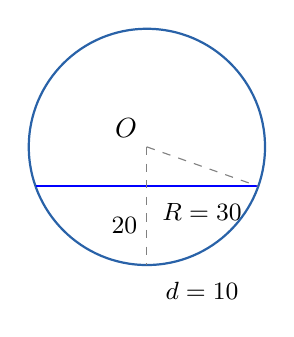
\begin{tikzpicture}[scale=0.05]
  \draw[thick, mainblue] (0,0) circle (30);
  % 水面
  \draw[thick, blue] (-28.28, -10) -- (28.28, -10);
  \fill (0,0) circle (2pt) node[above left]{$O$};
  \draw[dashed, gray] (0,0) -- (0, -30);
  \draw[dashed, gray] (0,0) -- (28.28, -10);
  \node[left, font=\small] at (0, -20) {$20$};
  \node[below, font=\small] at (14, -12) {$R=30$};
  \node[below, font=\small] at (14, -32) {$d=10$};
\end{tikzpicture}
\end{center}
\end{appbox}

\textbf{解：}

设圆心为 $O$，半径 $R = 30$ cm。水面为弦 $AB$。

设 $M$ 为 $AB$ 的中点，$OM \perp AB$。

积水深度为 $20$ cm（水面到管底），所以圆心到水面的距离：
\[
OM = 30 - 20 = 10 \text{（cm）}
\]

在直角三角形 $OMA$ 中：
\[
AM = \sqrt{OA^2 - OM^2} = \sqrt{900 - 100} = \sqrt{800} = 20\sqrt{2}
\]

水面宽度 $AB = 2 \times AM = 40\sqrt{2} \approx 56.57$ cm。

\begin{tipbox}[方法总结]
管道截面问题本质是圆的弦长计算。关键步骤：确定圆心到弦的距离（弦心距），再利用垂径定理和勾股定理求弦长。
\end{tipbox}

\vspace{6pt}

\begin{appbox}[【应用3】圆锥形烟囱帽]
一个圆锥形烟囱帽的底面直径为 $40$ cm，母线长为 $25$ cm。制作这个烟囱帽需要多少铁皮（不计接缝损耗）？侧面展开图的圆心角是多少度？
\end{appbox}

\textbf{解：}

底面半径 $r = 20$ cm，母线 $l = 25$ cm。

侧面积：
\[
S_{\text{侧}} = \pi r l = \pi \times 20 \times 25 = 500\pi \approx 1570.8 \text{（cm}^2\text{）}
\]

侧面展开图的圆心角：
\[
\theta = \frac{r}{l} \times 360° = \frac{20}{25} \times 360° = 288°
\]

需要铁皮约 $500\pi$ cm$^2$（约 $1570.8$ cm$^2$），侧面展开图的圆心角为 $288°$。

\begin{tipbox}[方法总结]
圆锥形物品的制作问题，关键是计算侧面积和展开图。注意：实际制作中还需要考虑接缝和损耗，但数学计算中一般忽略。
\end{tipbox}

% ==============================================================
% 第四部分：课堂练习
% ==============================================================
\section*{\textcolor{tipgreen}{四、课堂练习}}

\begin{enumerate}
  \item 在 $\odot O$ 中，弦 $AB = 6$，圆心到弦的距离为 $4$，求圆的半径。

  \item $AB$ 是 $\odot O$ 的直径，$C$、$D$ 是圆上的点，$\angle ABD = 50°$，求 $\angle ACD$。

  \item 四边形 $ABCD$ 内接于圆，$\angle A = 100°$，$\angle B = 80°$，求 $\angle C$ 和 $\angle D$。

  \item 已知 $\odot O$ 的半径为 $5$，点 $P$ 到圆心 $O$ 的距离为 $5$，则点 $P$ 在 $\odot O$ 的\blank{3cm}。

  \item 一个扇形的圆心角为 $60°$，半径为 $12$ cm，求扇形的弧长和面积。

  \item 一个圆锥的底面半径为 $4$ cm，高为 $3$ cm，求母线长、侧面积和全面积。

  \item 在 $\odot O$ 中，直径 $AB = 10$，弦 $CD = 6$，且 $AB \perp CD$ 于 $E$。求 $OE$ 的长（分两种情况讨论）。

  \item 正三角形的外接圆半径为 $6$，求正三角形的边长和面积。
\end{enumerate}

\vspace{10pt}

\begin{knowledgebox}[参考答案]

\textbf{1.} 由垂径定理，$AM = 3$。$r = \sqrt{3^2 + 4^2} = \sqrt{25} = 5$。

\medskip
\textbf{2.} $AB$ 是直径，$\angle ADB = 90°$。$\angle ABD = 50°$，所以 $\angle BAD = 40°$。$\angle ACD = \angle ABD = 50°$（同弧 $\widehat{AD}$ 上的圆周角相等）。

等等，让我重新分析。$\angle ACD$ 和 $\angle ABD$ 不一定在同弧上。让我重新考虑：

$\angle ABD = 50°$ 是弧 $\widehat{AD}$ 所对的圆周角。$\angle ACD$ 也是弧 $\widehat{AD}$ 所对的圆周角（$C$ 和 $B$ 在 $\widehat{AD}$ 的同一侧）。所以 $\angle ACD = \angle ABD = 50°$。

如果 $C$ 和 $B$ 在 $\widehat{AD}$ 的不同侧，则 $\angle ACD = 180° - 50° = 130°$。题目未明确，一般默认 $\angle ACD = 50°$。

\medskip
\textbf{3.} $\angle C = 180° - \angle A = 180° - 100° = 80°$。$\angle D = 180° - \angle B = 180° - 80° = 100°$。

\medskip
\textbf{4.} 点 $P$ 在 $\odot O$ 上（$d = r = 5$）。

\medskip
\textbf{5.} 弧长 $l = \dfrac{60 \times \pi \times 12}{180} = 4\pi$ cm。面积 $S = \dfrac{1}{2} \times 4\pi \times 12 = 24\pi$ cm$^2$。

\medskip
\textbf{6.} 母线 $l = \sqrt{r^2 + h^2} = \sqrt{16 + 9} = 5$ cm。侧面积 $= \pi \times 4 \times 5 = 20\pi$ cm$^2$。全面积 $= 20\pi + 16\pi = 36\pi$ cm$^2$。

\medskip
\textbf{7.} $R = 5$，$CD = 6$，$CN = 3$。$ON = \sqrt{25 - 9} = 4$。

情况一：$CD$ 在圆心一侧，$OE = 4$。

情况二：$CD$ 在圆心另一侧，$OE = 4$（距离取正值，结果相同）。

注意：若 $AB \perp CD$ 于 $E$，$E$ 为 $CD$ 的中点，则 $OE$ 就是弦心距 $= 4$。无需分情况。

\medskip
\textbf{8.} 正三角形的中心角 $= 120°$。边长 $a = 2R\sin 60° = 2 \times 6 \times \dfrac{\sqrt{3}}{2} = 6\sqrt{3}$。

边心距 $r = R\cos 60° = 6 \times \dfrac{1}{2} = 3$。

面积 $S = \dfrac{1}{2} \times 3a \times r = \dfrac{1}{2} \times 18\sqrt{3} \times 3 = 27\sqrt{3}$。

或用公式：$S = \dfrac{\sqrt{3}}{4}a^2 = \dfrac{\sqrt{3}}{4} \times 108 = 27\sqrt{3}$。

\end{knowledgebox}

\vfill
\begin{center}
\small\textcolor{gray}{本讲义仅供教学参考，例题可根据学生水平调整难度。}
\end{center}

\end{document}
